\documentclass[11pt]{article}
\usepackage{hyperref} 
\usepackage{amsmath, amsfonts, amssymb}
\usepackage{graphicx}
\usepackage{float}
\usepackage[margin=1in]{geometry}

\parindent0px

\emergencystretch=0pt
\pretolerance=150
\tolerance=10000
\hbadness=10000
\hfuzz=0pt

\title{Probability and Statistics by DeGroot Notes}
\author{Nathan Ueda}
\date{\today} 

\begin{document}
\maketitle 
\pagebreak
\tableofcontents 
\pagebreak

\section{Introduction to Probability}
\subsection{The History of Probability}
The use of probability to measure uncertainty and variability dates back hundredes of years.

\subsection{Interpretations of Probability}

\textbf{Probability Interpretations}
\begin{itemize}
    \item Frequency: If an experiment is carried out many times, the frequency with which a
    particular outcome occurred would define its probability.
    \item Classical: If an outcome of some experiment must be one of $n$ different, equally
    likely outcomes, the probability of each outcome is $\frac{1}{n}$.
    \item Subjective: An entity assigns probabilities to each possible outcome.
\end{itemize}

Probability theory does not depend on intepretation.

\subsection{Experiments and Events}

Probability allows us to quantify how likely an outcome is to occur. \\

\textbf{Experiments:} Any process in which the possible outcomes can be identified ahead of time.
\textbf{Events:} A well defined set of possible outcomes of the experiment (such as rolling an 
even number on a fair dice). \\

Although there is controversy in regard to the proper meaning and interpration of some of the
probabilities that are assigned to the outcomes of many experiements, once these probabilities
are assigned, there is complete agreemenet upon the mathematical theory of probability. \\

Almost all work in the mathematical theory of probability is related to:
\begin{itemize}
    \item Methods for determining probabilities of certain events from given probabilities for
    each possible outcome in an experiment.
    \item Methods for revising probabilities of events when additional relevant information is 
    obtained.
\end{itemize}

\subsection{Set Theory}

\textbf{Sample Space:} The collection of all possible outcomes of an experiment. \\
\textbf{Empty Set:} Subset of $S$ containing no elements, denoted $\emptyset$, representing
any events that cannot occur. \\
\textbf{Complement:} For some set $A$, its complement, denoted $A^c$, is the set containing all 
elements of $S$ not in $A$. \\
\textbf{Union:} For $n$ sets $A_1, \ldots, A_n$, their union, denoted $A_1 \cup \ldots \cup A_n
$ or $ \bigcup_{i=1}^{n} A_i $, is defined as the set containing all outcomes that belong to at
least one of these $n$ sets. \\
\textbf{Intersection:} For $n$ sets $A_1, \ldots, A_n$, their intersection, denoted $A_1 \cap 
\ldots \cap A_n $ or $ \bigcap_{i=1}^{n} A_i $, is defined as the set containing the elements 
common to all these $n$ sets. \\
\textbf{Disjoint/Mutually Exclusive:} Two sets $A$ and $B$ are disjoint/mutually exclusive if 
they have no outcomes in common, that is, if $ A \cap B = \emptyset $, representing that both
$A$ and $B$ cannot occur.

\subsection{The Definition of Probability}

Axioms of Probability:
\begin{enumerate}
    \item For every event $A$, $P(A) \ge 0$.
    \item $P(S) = 1$.
    \item $P( \bigcup_{i=1}^{\infty} A_i) = \sum_{i=1}^{\infty}P(A_i)$.
\end{enumerate}

Basic Theorems:
\begin{enumerate}
    \item $P(\emptyset) = 0$.
    \item For every finite sequence of $n$ disjoint events, $A_1, \ldots, A_n$, $P( 
    \bigcup_{i=1}^{n} A_i) = \sum_{i=1}^{n}P(A_i)$.
    \item For every event $A$, $P(A^c) = 1 - P(A)$.
    \item If $A \subset B$, then $P(A) \le P(B)$.
    \item For every event $A$, $0 \le P(A) \le 1$.
    \item For every two events $A$ and $B$, $P(A \cap B^c) = P(A) - P(A \cap B)$.
    \item For every two events $A$ and $B$, $P(A \cup B) = P(A) + P(B) - P(A \cap B)$.
    \item Bonferroni Inequality: For all events $A_1, \ldots, A_n$, $P(\bigcap_{i=1}^{n} A_i) 
    \ge 1 - \sum_{i=1}^{n} P(A_i^c)$.
\end{enumerate}

\subsection{Finite Sample Spaces}

Simple Sample Space
\begin{itemize}
    \item Has a finite number ($n$) of possible outcomes.
    \item Each outcome has an equal probability ($\frac{1}{n}$).
    \item If an event $A$ has $m$ outcomes, then $P(A) = \frac{m}{n}$.
\end{itemize}

\subsection{Counting Methods}

\textbf{Multiplication Rule:} An experiment with $k$ parts where the $i$th part has $n_i$ 
possible outcomes (regardless of which specific outcomes have occurred in the other parts) has 
a sample space $S = n_1 n_2 \ldots n_k$. \\

\textbf{Permutations ($P_{n,k}$):}
\begin{itemize}
    \item Number of ways to arrange a set (order matters).
    \item Sampling considering $n$ different items and making $k$ choices from them.
    \begin{itemize}
        \item Sampling with replacement: $n^k$.
        \item Sampling without replacement: $n(n-1) \ldots (n-k+1)$.
        \begin{itemize}
            \item $n$ options for first choice, $n-1$ options for second choice, $n-k+1$ 
            options for $k$th choice.
        \end{itemize}
    \end{itemize}
    
    \item The number of permutations of $n$ different items is $P_{n,n} = n$!.
    \item The number of permutations of $n$ different items making $k$ choices ($0 \le k \le 
    n$) is
        \[P_{n,k} = n(n-1) \ldots (n-k+1)\]
        \[P_{n,k} = n(n-1) \ldots (n-k+1) \left(\frac{1}{1}\right)\]
        \[P_{n,k} = n(n-1) \ldots (n-k+1) \left(\frac{(n-k)(n-k-1) \ldots 1}{(n-k)(n-k-1) 
        \ldots 1}\right)\]
        \[P_{n,k} = \frac{n(n-1) \ldots (n-k+1)(n-k)(n-k-1) \ldots 1}{(n-k)(n-k-1) \ldots 1}\]
        \[P_{n,k} = \frac{n!}{(n-k)!}\]
\end{itemize}

\subsection{Combinatorial Methods}
\textbf{Combinations ($C_{n,k}$):}
\begin{itemize}
    \item Number of subsets (order does not matter).
    \item Permutations may be thought of as combinations of size $k$ chosen out of $n$, 
    multiplied by the number of ways to arrange the size $k$ subsets, $k$!. More formally, this
    says 
    \[ P_{n,k} = C_{n,k} k!\]
    \item Combinations (binomial coefficient) are the number of distinct subsets of size $k$ 
    that can be chosen from a set of size $n$ (this is the same formula as for permutations,
    except we are dividing out the number of ways we can rearrange the subsets, $k$!, since 
    order does not matter): 
        \[C_{n,k} = {n \choose k} = \frac{P_{n,k}}{k!} = \frac{\frac{n!}{(n-k)!}}{k!} =  \frac{n!}{(n-k)!k!} \]
    \item Combinations without replacement: ${n+k-1 \choose k}$.
\end{itemize}

\subsection{Multinomial Coefficients}

The total number of different ways of dividing $n$ elements into $k$ groups is 
\[ {n \choose n_1, n_2, \ldots, n_k} = {n \choose n_1} {n - n_1 \choose n_2} {n - n_1 - n_2 
\choose n_3} \cdots {n - n_1 - \cdots - n_{k-2} \choose n_{k-1}} = \frac{n!}{n_1!n_2! \cdots 
n_k!}\]

\subsection{The Probability of a Union of Events}

\begin{itemize}
    \item Union of two events $A_1$ and $A_2$: \[P(A_1 \cup A_2) = P(A_1) + P(A_2) - P(A_1 \cap
    A_2)\]
    \item Union of three events $A_1$, $A_2$, and $A_3$: \[P(A_1 \cup A_2 \cup A_3) = P(A_1) + 
    P(A_2) + P(A_3) - \left[ P(A_1 \cap A_2) + P(A_1 \cap A_3) + P(A_2 \cap A_3) \right] \] \[ 
    + P(A_1 \cap A_2 \cap A_3)\]
    \item Union of $n$ events $A_1, \ldots, A_n$: \[ P \left(\bigcup_{i=1}^{n} A_i\right) = 
    \sum_{i=1}^{n} P(A_i) - \sum_{i<j}P(A_i \cap A_j) + \sum_{i<j<k}P(A_i \cap A_j \cap A_k) -
    \] \[ \sum_{i<j<k<l} P(A_i \cap A_j \cap A_k \cap A_l) + \cdots + {(-1)}^{n+1} P(A_1 \cap 
    A_2 \cap \cdots \cap A_n)\]
\end{itemize}

\section{Conditional Probability}

\subsection{The Definition of Conditional Probability}

\begin{itemize}
    \item Conditional probability is the updating of probabilities when certain events are
    observed.
    \item The updated probability of event $A$ after we learn that event $B$ has occured is the
    conditional probability of $A$ given $B$, denoted $P(A|B)$.
    \item When we go from $P(A)$ to $P(A|B)$, we say we are conditioning on $B$.
    \item For $P(B) > 0$ \[P(A|B) = \frac{P(A \cap B)}{P(B)}\].
    \item Intuitively, this is saying the probability of $A$ occurring, given $B$ has occurred
    is equal to the outcomes where both $A$ and $B$ occurred (which makes sense since we know 
    $B$ has occurred and we want to find the probability of $A$ also occurring) divided by the 
    probability of $B$ occurring (which makes sense since we know $B$ occurred, we can 
    renormalize the sample space to only contain outcomes where $B$ occurred).
\end{itemize}

\textbf{Multiplication Rule for Conditional Probabilities}
\begin{itemize}
    \item For 2 events $A,B$
    \begin{itemize}
        \item If $P(B) > 0$ \[P(A \cap B) = P(B)P(A|B)\]
        \item If $P(A) > 0$ \[P(A \cap B) = P(A)P(B|A)\]
    \end{itemize}
    \item For $n$ events $A_1, \ldots, A_n$ such that $P(A_1 \cap \ldots \cap A_{n-1}) > 0$ 
    \[P(A_1 \cap \ldots \cap A_n) = P(A_1)P(A_2|A_1)P(A_3|A_1 \cap A_2) \ldots P(A_n|A_1 \cap
    \ldots A_{n-1})\]
    \item For $n$ events $A_1, \ldots, A_n, B$ such that $P(B) > 0$ and $P(A_1 \cap \ldots \cap
    A_{n-1}) > 0$ 
    \[P(A_1 \cap \ldots \cap A_n|B) = P(A_1|B)P(A_2|A_1 \cap B)P(A_3|A_1 \cap A_2 \cap B) 
    \ldots P(A_n|A_1 \cap \ldots A_{n-1} \cap B)\]
\end{itemize}

\textbf{Law of Total Probability}
\begin{itemize}
    \item Tells us that to get the unconditional probability of $A$, we can divide the sample
    space into disjoint slices $B_j$, find the conditional probability of $A$ within each of 
    these slices, then take a weighted sum of the conditional probabilities, where the weights
    are the probabilities $P(B_j)$.
    \item Often used in tandum with Bayes' Rule.
    \item Relates conditional probability to unconditional probability .
    \item Partition: Let $S$ denote the sample space and consider $k$ events $B_1, \ldots, B_k$
    in $S$ such that $B_1, \ldots, B_k$ are disjoint and $\bigcup_{i=1}^{k}B_i = S$. Then 
    events $B_1, \ldots, B_k$ form a partition in $S$. In other words, only one of these events
    can occur and combined they fill the entire sample space.
    \item Suppose events $B_1, \ldots, B_k$ form a partition of the space $S$ and $P(B_j) > 0$
    for $j = 1, \ldots, k$. Then \[P(A) = \sum_{j=1}^{k} P(B_j \cap A) = \sum_{j=1}^{k} P(B_j)
    P(A|B_j)\].
    \item Conditional LOTP \[P(A|C)= \sum_{j=1}^{k}P(B_j|C)P(A|B_j \cap C)\].
\end{itemize}

\subsection{Independent Events}

\textbf{Independence of 2 Events:}
\begin{itemize}
    \item Two events are independent if learning that one occurred does not change the
    probability of the other event.
    \item Two events $A$ and $B$ with positive probabilities are independent if 
    \[P(A \cap B) = P(A)P(B)\] 
    \item Similarly, two events $A$ and $B$ with positive probabilities are independent if 
    \[P(A|B) = P(A) \text{ and } P(B|A)=P(B)\]
    \item If two events $A$ and $B$ are independent, then $A$ and $B^C$ are independent
\end{itemize}

\textbf{Independence of k Events:}
\begin{itemize}
    \item For $k$ events, if knowing what happened with any particular subset of the events 
    gives us no information about what happened with the events not in the subset, the events
    are independent.
    \item $k$ events are (mutually) independent if 
    \begin{itemize}
        \item Any pair $P(A_i \cap A_j) = P(A_i)P(A_j) \text{ for } i \ne j$ 
        \item Any triplet $P(A_i \cap A_j \cap A_k) = P(A_i)P(A_j)P(A_k) \text{ for } i \ne j 
        \ne k$
        \item $\ldots$
        \item The n-tuplet $P(A_1 \cap \ldots \cap A_n) = P(A_1) \ldots P(A_n) $
    \end{itemize}
\end{itemize}

When deciding whether or not to model events as independent, try to answer the following 
question: ``If I were to learn that some of these events occurred, would I change the 
probabilities of any of the others?'' \\

\textbf{Conditional Independence:}
\begin{itemize}
    \item Two events $A$ and $B$ are conditionally independent given $E$ if $P(A \cap B|E) =
    P(A|E)P(B|E)$.
    \item It is defined as independence but with respect to the conditional probabilities.
\end{itemize}

\subsection{Bayes' Theorem}

\begin{itemize}
    \item Bayes' Theorem relates $P(A|B)$ to $P(B|A)$.
    \item This is important as often it is easier to solve either $P(A|B)$ or $P(B|A)$.
    \item Suppose that we are interested in which of several disjoint events $A_1, \ldots, A_k$
    will occur and that we will get to observe some other event $B$. If $P(B|A_i)$ is available
    for each $i$, then Bayes' theorem is a useful formula for computing the conditional 
    probabilities of the $A_i$ events given $B$, that is, $P(A_i|B)$ for each $i$.
\end{itemize}


\textbf{Bayes' Theorem for 2 Events}
\begin{itemize}
    \item \[P(A|B) = \frac{P(B|A)P(A)}{P(B)}\]
    \item It is often common to use LOTP in the denominator
    \[P(A|B) = \frac{P(B|A)P(A)}{\sum_{i=1}^{n}P(B|A_i)P(A_i)} = 
    \frac{P(B|A)P(A)}{P(B|A)P(A) + P(B|A^c)P(A^c)} \]
\end{itemize}



\textbf{Bayes' Theorem for $n$ Events}

\[P(A_i|B)=\frac{P(B|A_i)P(A_i)}{\sum_{j=1}^{n}P(B|A_j)P(A_j)}\]

\textbf{Prior vs. Posterior Probabilities}
\begin{itemize}
    \item Prior probabilities represent probabilities \textit{before} new evidence is 
    introduced.
    \begin{itemize}
        \item $P(A)$
    \end{itemize}
    \item Posteror probabilities represent probabilities \textit{after} the new evidence in 
    taken into consideration.
    \begin{itemize}
        \item $P(A|B)$
    \end{itemize}
\end{itemize}

\textbf{Conditional Version of Bayes' Theorem}
\[P(A_i|B \cap C) = \frac{P(B|A_i \cap C)P(A_i|C)}{\sum_{j=1}^{n}P(B|A_j \cap C)P(A_j|C)}\]

\subsection{The Gambler's Ruin Problem}

\textbf{High Level Problem Overview:} Consider two gamblers with finite resources who 
repeatedly play the same game against each other. Using the tools of conditional probability, 
we can calculate the probability that each of the gamblers will eventually lose all of his 
money to the opponent. As this game ends only when one of the gamblers has no money left, this
problem is fittingly called, the Gambler's Ruin problem. \\

\textbf{Problem Statement}
\begin{itemize}
    \item Two gamblers, $A$ and $B$, make \$1 bets each round.
    \item $A$ has a probability $p$ of winning, $B$ has probability $1-p$ of winning.
    \item $A$ starts with $k$ dollars, $B$ starts with $k-i$ dollars, for a combined fortune of
    $k$.
    \item The game continues until one of the gamblers has 0 dollars left.
    \item The goal is to determine the probability that $A$ will reach $k$ dollars before 0.
\end{itemize}

\section{Random Variables and Distributions}
\subsection{Random Variables and Discrete Distributions}

\textbf{Random Variables}
\begin{itemize}
    \item A function that maps each outcome in the sample space to the real line.
    \item Two main types of random variables: discrete and continuous random variables.
    \item Main tool used for modeling unknown quantities in statistical analysis.
\end{itemize}

\textbf{Distributions}
\begin{itemize}
    \item A distribution specifies the probabilities of all events associated with a random
    variable (maps outcomes to probabilities).
\end{itemize}

\textbf{Discrete Distributions}
\begin{itemize}
    \item Distributions that assign positive probability to at most countably many different
    values.
    \item Discrete distributions can be characterized by its probability function (p.f.) aka
    probability mass function (p.m.f).
\end{itemize}

\textbf{Discrete Random Variables}
\begin{itemize}
    \item A random variable with a discrete distribution.
    \item Is a discrete r.v. if the r.v. can take only a finite number $k$ of different values
    $x_1, \ldots x_k$ or, at most, an infinite sequence of different values $x_1, x_2, \ldots $
\end{itemize}

\textbf{Probability Function}
\begin{itemize}
    \item A function that describes the probabilities of different values of a r.v.
    \item For a discrete r.v., the p.f. of $X$ is defined as the function $f$ such that for 
    every real number $x$, \[f(x)=P(X=x)\]
    \item If $x$ is not a possible value of $X$, then $f(x)=P(X=x)=0$
    \item The support of $X$ is all values $x$ such that $f(x)=P(X=x)>0$.
    \item To be a valid p.f.
    \begin{itemize}
        \item The probabilities of all possible outcomes of $X$ sum to 1. More formally, if the
        sequence $x_1, x_2, \ldots$ includes all the possible values of $X$, then $\sum_{i=1}^
        {\infty} f(x_i) = 1$.
        \item All possible values of $X$ have a probability greater than 0 and all other values 
        have a probability of 0.
    \end{itemize}
    \item A p.f. is only for discrete distributions.
\end{itemize}

\textbf{Example}
    \begin{itemize}
        \item In an experiment in which a fair coin is tossed 2 times, we can define a random 
        variable $X$ to represent the number of heads in each outcome.
        \item The possible outcomes in the sample space are $S = \{TT, HT, TH, HH\}$.
        \item $X(TT)=0,\ X(TH)=1,\  X(HT)=1,\ X(HH)=2$.
        \item Therefore, the p.f. of $X$ is the function $f$ given by 
        \begin{itemize}
            \item $f(0) = P(X=0) = 1/4 $
            \item $f(1) = P(X=1) = 1/2 $
            \item $f(2) = P(X=2) = 1/4 $
        \end{itemize}
    \end{itemize} 

\textbf{Common Named Distributions}
\begin{itemize}
    \item Some random variables has distributions that occur so frequently they are given 
    names. 
    \item These common named distributions represent a family of distributions (for example, 
    there are a family of Bernoulli distributions, not just one). What allows us to determine 
    the specific distribution we have (the specific Bernoulli distribution we have), are 
    parameters (for Bernoulli, this is the value for $p$)
\end{itemize}

\textbf{Bernoulli Distributions}
\begin{itemize}
    \item A distribution of the probabilities of a single experiment asking a yes-no question.
    \item A r.v. $X$ that takes on only two values 1 and 0 (success and failure).
    \item Has one parameter, $p$.
    \item Written $X \sim \text{Bern}(p)$.
    \item p.f. of $X$
    \[ P(X=x) = f(x) = \begin{cases} 
        p & \text{for } x=1 \\
        1-p & \text{for } x=0 \\
        0 & \text{otherwise}
     \end{cases}
  \]
\end{itemize}

\textbf{Discrete Uniform Distributions}
\begin{itemize}
    \item A distribution where each outcome for the r.v. has an equally likely probability.
    \item A r.v. $X$ where, for 2 integers $a,b$ where $a \le b$, the value of $X$ is equally 
    likely to be each of the integers $a, \ldots, b$.
    \item A uniform distribution on a set of $k$ integers has probability of $1/k$ on each 
    integer.
    \item Has two parameters, $a,b$.
    \item Written $X \sim \text{DUnif}(a,b)$.
    \item p.f. of $X$
    \[ P(X=x) = f(x) = \begin{cases} 
        \frac{1}{b-a+1} & \text{for } x=a, \ldots, b \\
        0 & \text{otherwise}
     \end{cases}
  \]
\end{itemize}

\textbf{Binomial Distributions}
\begin{itemize}
    \item A distribution that is based upon a r.v. denoting the number of successes in $n$ 
    independent Bernoulli trials (an experiment that can end only in success or failure).
    \item Suppose that $n$ independent Bernoulli trials  are performed, each with success 
    probability $p$. If we let $X$ be the number of success, then the distribution of $X$ is 
    called the Binomial distribution with parameters $n$ and $p$. 
    \item Has two parameters, $n, p$.
    \item Written $X \sim \text{Bin}(n,p)$.
    \item p.f. of $X$
    \[ P(X=x) = f(x) = \begin{cases} 
        {n \choose x}p^x{(1-p)}^{n-x} & \text{for } x=0, \ldots, n \\
        0 & \text{otherwise}
     \end{cases}
  \]
  \begin{itemize}
    \item The probability of obtaining exactly $x$ successes and $n-x$ failures is $p^x{(1-p)}
    ^{n-x}$. Since there are ${n \choose x}$ ways of ordering this, its follows that $P(X=x)=
    {n \choose x}p^x{(1-p)}^{n-x}$.
  \end{itemize}
  \item The Bernoulli distribution is just a special case of the Binomial distribution where 
  $n=1$, that is, Bin$(1, p)$.
\end{itemize}

\subsection{Continuous Distributions}

\textbf{Continuous Distributions}
\begin{itemize}
    \item Distributions that have a range of values that are uncountably infinite. 
    \item Continuous distributions can be characterized by its probability density function 
    (p.d.f.)
    \item Assign probability 0 to individual values, that is, $P(X=x)=0$ for every number $x$.
\end{itemize}

\textbf{Continuous Random Variables}
\begin{itemize}
    \item A random variable with a continuous distribution.
\end{itemize}

\textbf{Probability Density Function}
\begin{itemize}
    \item A nonnegative function $f$ for a r.v. $X$ such that the integral of $f$ over each 
    interval $[a,b]$ gives the probability that $X$ is in the interval, that is, $P(a \le X 
    \le b) = \int_{a}^{b} f(x) \,dx$.
    \item Similarly, $P(X \ge a) = \int_{a}^{\infty} f(x) \,dx$ and $P(X \le b) = \int_
    {-\infty}^{b} f(x) \,dx$.
    \item Density is not probability (density can be greater than 1). The p.d.f. of $X$, 
    $f(x)$, itself is not the probability that $X$ is near $x$, instead, the integral of $f$ 
    over values near x gives the probability that $X$ is near $x$, and the integral is never 
    greater than 1.
    \item Since the endpoints have probability 0, for an interval $(a,b)$, $P(a < X < b) = 
    P(a \le X \le b) = P(a < X \le b) =  P(a \le X < b)$
    \item The support of $X$ is all values $x$ such that $f(x)=P(X=x)>0$.
    \item To be a valid p.d.f.
    \begin{itemize}
        \item The p.d.f. of $X$ must integrate to 1, that is, $\int_{-\infty}^{\infty} f(x) \,dx=1$.
        \item For all $x$, $f(x) \ge 0$.
    \end{itemize}
    \item To get a desired probability, integrate the p.d.f. over the appropriate range.
    \item In general, we can think of $f(x) \,dx$ as the probability of $X$ being in an 
    infinitesimally small interval containing $x$, of length $\,dx$,
\end{itemize}

\textbf{Uniform Distributions}
\begin{itemize}
    \item A Uniform r.v. on the interval $(a,b)$ is a completely random number, which speicifies 
    that the p.d.f. is constant over the interval.
    \item Has two parameters, $a,b$.
    \item Written $X \sim \text{Unif}(a,b)$.
    \item p.d.f. of $X$
    \[ f(x) = \begin{cases} 
        \frac{1}{b-a} & \text{for } a \le x \le b \\
        0 & \text{otherwise}
     \end{cases}
  \]
\end{itemize}

\textbf{Normalizing Constants}
\begin{itemize}
    \item Often, we will have a p.d.f without a specified value for $c$, 
    the normalizing constant. 
    \item This happens especially often when we find sampling distributions 
    of summaries of observed data where we can determine the p.d.f of a 
    r.v. except for the constant factor.
    \item The constant is unique.
    \item Using the fact that the p.d.f must integrate to 1, we can solve 
    for $c$.
    \item Example:
    \[\int_{0}^{4}cx \,dx = 1\]
    \[c\int_{0}^{4}x \,dx = 1\]
    \[c\frac{x^2}{2}\rvert_0^4 = 1\]
    \[c\left(\frac{4^2}{2}-0\right)= 1\]
    \[c\left(\frac{16}{2}\right)= 1\]
    \[8c= 1\]
    \[c= \frac{1}{8}\]
\end{itemize}

\subsection{The Cumulative Distribution Function}   

\textbf{Cumulative Distribution Function}
\begin{itemize}
    \item A function of a r.v. $X$, denoted $F$, that gives the probability that the r.v. is 
    less than or equal to $x$ \[F(x)=P(X \le x) \text{ for } -\infty < x < \infty\]
    \item While a p.f is defined only for discrete r.v.s and a p.d.f is defined for only 
    continuous r.v.s, a c.d.f. is defined for both discrete and continuous r.v.'s.
    \item The c.d.f. is another way of characterizing the distribution of a r.v.
    \item The value of $F$ at every point $x$ must be a number $F(x)$ in the interval $[0,1]$
    because $F(x)$ is the probability of the event ${X \le x}$.
    \item For every value $x$
    \[P(X > x) = 1 - F(x)\]
    \item For all values $x_1$ and $x_2$ such that $x_1 < x_2$
    \[P(x_1 < X \le x_2) = F(x_2) - F(x_1)\]
    \item For each value $x$
    \[P(X < x) = F(x^-)\]
    \item For every value $x$
    \[P(X=x) = F(x) - F(x^-)\]
    \begin{itemize}
        \item For every value $x$, $P(X=x)$ is equal to the amount of the jump that occurs in 
        $F$ at the point $x$. If $F$ is continuous at that point $x$, that is, if there is no 
        jump in $F$ at $x$ ($F(x^-)=F(x^+)=F(x)$), then $P(X=x)=0$.
    \end{itemize}
\end{itemize}

\textbf{CDF Properties}
\begin{itemize}
    \item Nondecreasing: If $x_1 \le x_2$, then $F(x_1) \le F(x_2)$.
    \item Convergence to 0 and 1 in the limits
    \[ \lim_{x \to -\infty} F(x)=0 \]
    \[ \lim_{x \to \infty} F(x)=1 \]
    \item Right continuous: A c.d.f. is continuous except for the possibility of having some 
    jumps. If there are jumps, the c.d.f. is continuous from the right
    \[F(x) = F(x^+)\] at every point $x$.
\end{itemize}

\textbf{CDF of a Discrete Distribution}
\begin{itemize}
    \item $F(x_i)$ will have a jump of magnitude $f(x_i) = P(X = x_i)$ at each possible value $x_i$ of $X$.
    \item $F(x)$ will be constant and horizontal between every pair of successive jumps. If the 
    interval $[a,b]$ represents this constant area between successive jumps, then $P(a < X < b)
    = 0$.
\end{itemize}

\textbf{CDF of a Continuous Distribution}
\begin{itemize}
    \item If $X$ is a continuous r.v., $f(x)$ is its p.d.f, and $F(x)$ is its c.d.f., then $F$
    is continuous at every $x$,
    \[F(x) = \int_{-\infty}^{x} f(t) \,dt\] and \[\frac{dF(x)}{dx} = f(x)\] 
    at all $x$ such that $f$ is continuous.
    \item The c.d.f. of a continuous r.v. $X$ can be obtained from the p.d.f and vice versa.
    \begin{itemize}
        \item The p.d.f is the derivative of the c.d.f.
        \[f(x) = F'(x)\]
        \item The c.d.f. is an antiderivative (a function whose derivative is the original 
        function) of the p.d.f.
    \end{itemize}
\end{itemize}

\textbf{Quantile Function}
\begin{itemize}
    \item A percentile is a way of expressing where an observation falls in a range of other 
    observations. It is the value below which a percentage of data falls (divides the data into
    hundreths).
    \item If we are looking for the $100p$ ($p$ is strictly between 0 and 1) percentile.
    of a r.v. $X$ with a c.d.f. $F$, the inverse of $F$, $F^{-1}(p)$ allows us to do so.
    \item The $p$ quantile of $X$, $F^{-1}(p)$, is the smallest value $x$ such that $F(x) \ge p$.
    \item The quantile function, $F^{-1}$, is defined on the open interval $(0,1)$.
    \item Exists for discrete and continuous distributions.
    \item Certain quantiles have certain names
    \begin{itemize}
        \item Lower quartile: 25th percentile
        \item Median: 50th percentile
        \item Upper quartile: 75th percentile
    \end{itemize}
    \item The quantile function is an alternative way to characterize a distribution.
    \item To find the quantile function $F^{-1}(p)$ when we know the c.d.f., we can set $F(x)=p$ and 
    solve for $x$.
\end{itemize}

\subsection{Bivariate Distributions}

\textbf{Joint/Bivariate Distribution Basics}
\begin{itemize}
    \item Often, in real life we are interested in several r.v.s that are related to each 
    other. For example, if studying a random family, we may want to study the number of people
    in the family (which would be one r.v.) and the household income (which would be another
    r.v.). Joint distributions allow us to assign probabilities to these events.
    \item A joint distribution of two r.v.s $X$ and $Y$ is the collection of all probabilities 
    of the form $P[(X,Y) \in C]$ for all sets $C$ of pairs of real numbers such that $\{(X, Y)
    \in C\}$ is an event.
\end{itemize}

\textbf{Discrete Joint Distribution}
\begin{itemize}
    \item Let $X$ and $Y$ be random variables, and consider the ordered pair $(X,Y)$. If there
    are only finitely or at most countably many different possible values $(x,y)$ for the pair 
    $(X,Y)$, then we say that $X$ and $Y$ have a discrete joint distribution.
\end{itemize}

\textbf{Joint Probability Function}
\begin{itemize}
    \item The joint p.f. of discrete r.v.s $X$ and $Y$ is the function $f$, such that for every 
    point $(x,y)$ in the $xy$-plane
    \[f(x,y)=P(X=x, Y=y)\]
    where $f(x,y)$ is the probability of $x$ and $y$ occurring.
    \begin{figure}[H] 
        \centering 
        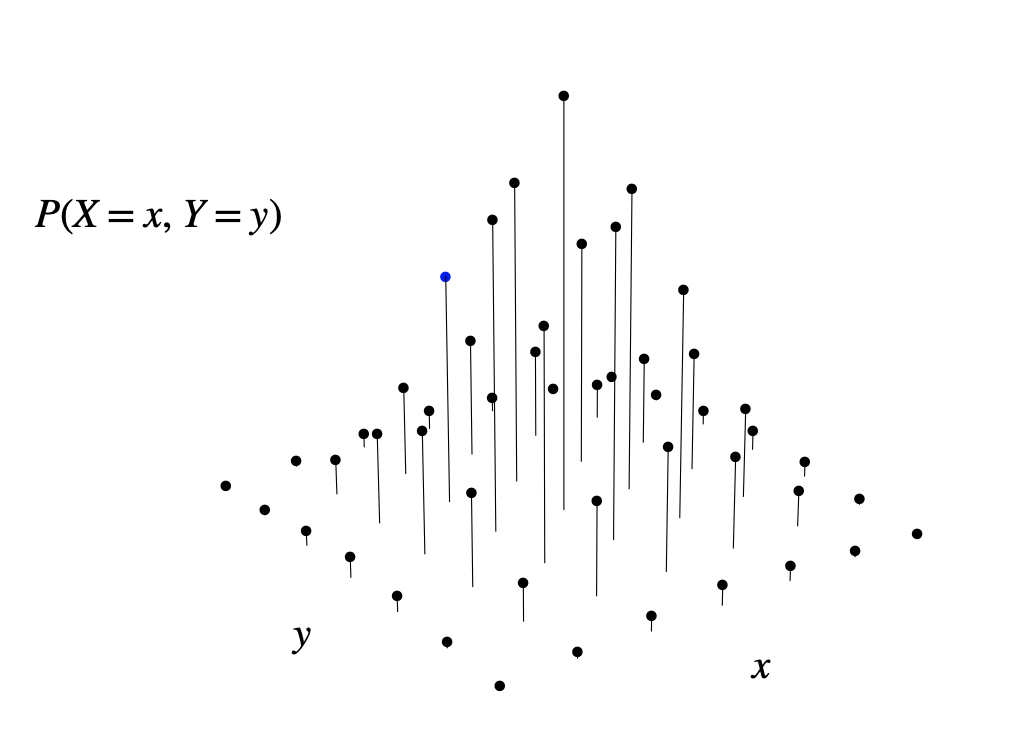
\includegraphics[width=3in]{imgs/joint_pf.png}
        \caption{Joint p.f. of discrete r.v.s $X$ and $Y$. The height of a vertical bar at 
        $(x,y)$ represents the probability $P(X=x, Y=y)$. The total summed heights of the vertical
        bars must be 1.}
    \end{figure}
    \item To be a valid joint p.f.
    \begin{itemize}
        \item The probabilities of all possible outcomes of $(X,Y)$ sum to 1. That is
        \[\sum_{\text{All } (x,y)} f(x,y) = 1\]
        \item All possible values of $(X,Y)$ have a probability greater than 0 and all other 
        values have a probability of 0. That is, if $(x,y)$ is not one of the possible values 
        of $(X,Y)$, then $f(x,y)=0$.
    \end{itemize}
    \item We can find the probability of the event $(X,Y) \in C$ for any set $C$ of points 
    (ordered pairs) in the support of $(X,Y)$ by summing over the joint p.f. over $C$
    \[P[(X,Y) \in C] = \sum_{(x,y) \in C} f(x,y)\]
\end{itemize}

\textbf{Continuous Joint Distribution}
\begin{itemize}
    \item Two r.v.s $X$ and $Y$ have a continuous joint distribution if there exists a 
    nonnegative function $f$ (joint p.d.f.) defined over the entire $xy$-plane such that for 
    every subset $C$ of the plane, 
    \[P[(X,Y) \in C] = \int_C \int f(x,y) \,dxdy\]
    if the integral exists.
\end{itemize}

\textbf{Joint Probability Density Function}
\begin{itemize}
    \item If $X$ and $Y$ are continuous r.v.s with joint c.d.f $F(x,y)$, their joint p.d.f. is 
    the derivative of the joint c.d.f. with respect to $x$ and $y$ (take the derivative of $y$
    treating $x$ as a constant, then take the derivative of $x$ treating $y$ as a constant)
    \[ f(x,y) = \frac{\partial^2}{\partial x \partial y} F(x,y) \]
    \begin{figure}[H] 
        \centering 
        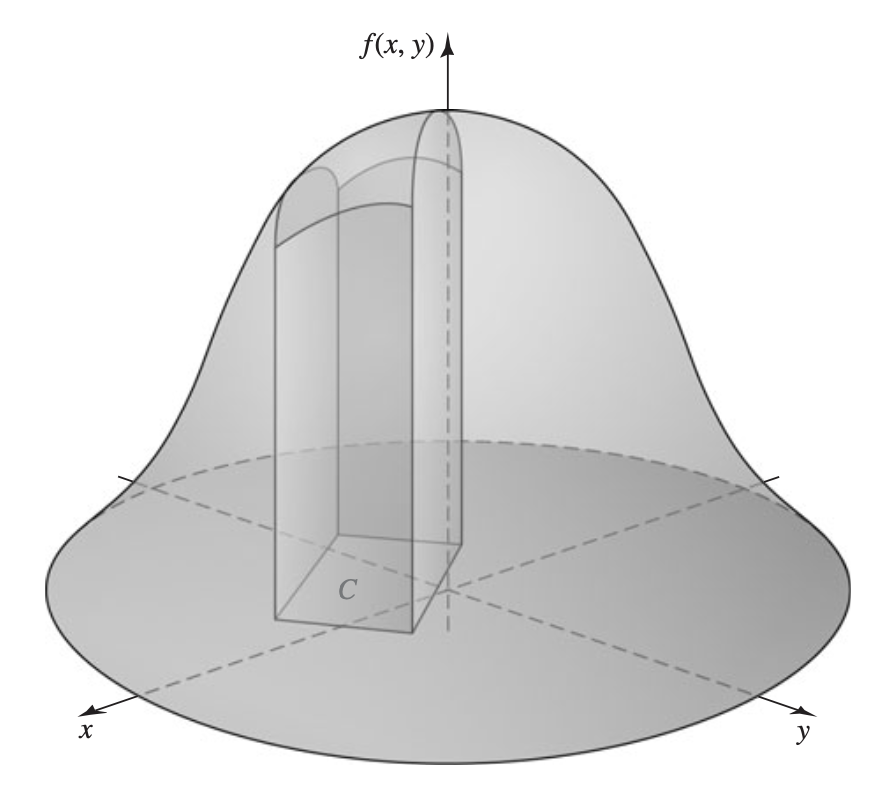
\includegraphics[width=3in]{imgs/joint_pdf.png}
        \caption{Joint p.d.f. of continuous r.v.s $X$ and $Y$. When integrating over the region 
        $C$, we are calculating the volume under the surface of the joint p.d.f and above $C$.
        The total volume under a valid joint p.d.f. is 1.}
    \end{figure}
    \item To be a valid joint p.d.f.
    \begin{itemize}
        \item The joint p.d.f. of $X$ and $Y$ must integrate to 1, that is, $\int_{-\infty}^{\infty}
        \int_{-\infty}^{\infty} f(x,y) \,dxdy =1$.
        \item For all $x$, $f(x) \ge 0$.
    \end{itemize}
\end{itemize}

\textbf{Mixed Bivariate Distributions}\
\begin{itemize}
    \item Sometimes, we must consider a mixed bivariate distribution in which we have one 
    discrete r.v. and one continuous r.v.
\end{itemize}

\textbf{Joint Probability Function/Probability Density Function}
\begin{itemize}
    \item Let $X$ and $Y$ be r.v.s such that $X$ is discrete and $Y$ is continuous. Suppose 
    that there is a function $f(x,y)$ (join p.f./p.d.f. of $X$ and $Y$) defined on the $xy$-
    plane such that, for every pair $A$ and $B$ of subsets of the real numbers,
    \[P(X \in A, Y \in B) = \int_B \sum_{x \in A} f(x,y) \,dy\]
    if the integral exists.
\end{itemize}

\textbf{Joint Cumulative Distribution Function}
\begin{itemize}
    \item The joint c.d.f. of two continuous r.v.s $X$ and $Y$ is define as the function $F$ such 
    that for all values of $x$ and $y$ $(-\infty < x < \infty, -\infty < y < \infty)$ 
    \[F(x,y)=P(X \le x, Y \le y) = \int_{-\infty}^{y} \int_{-\infty}^{x} f(r,s) \,drds\]
    \item The probability that an event occurs such that $X \le x$ and $Y \le y$.
\end{itemize}

\subsection{Marginal Distributions}

\textbf{Marginal Distributions}
\begin{itemize}
    \item A marginal distribution is simply distribution of any 1 r.v.
    \item Often, we may start with a joint distribution of 2 r.v.s and want to find the 
    distribution of just 1 of them.
    \item The distribution of 1 r.v. $X$ computed from a joint distribution is called the 
    marginal distribution of $X$. 
    \item Each r.v. will have a marginal c.d.f. as well as a marginal p.d.f or p.f.
    \item The name marginal distribution derives from the fact that the marginal distribution
    are the totals that appear in the margins of tables. 
\end{itemize}

\textbf{Marginal Probability Function}
\begin{itemize}
    \item For discrete r.v.s $X$ and $Y$ that have a joint p.f. $f$, the marginal p.f., $f_1$,
    of $X$ is 
    \[ f_1(x) = P(X=x)= \sum_{\text{All } y} P(X=x, Y=y) = \sum_{\text{All } y} f(x,y) \]
    which says, to find the marginal p.f. of $X$, hold the 1 value of $x$ fixed and then sum 
    over all the outcomes of $Y$.
    \item Similarly, if $f_2$ is the marginal p.f. of $Y$
    \[ f_2(y) = P(Y=y)= \sum_{\text{All } x} P(X=x, Y=y) = \sum_{\text{All } x} f(x,y) \]

\end{itemize}

\textbf{Marginal Probability Density Function}
\begin{itemize}
    \item For continuous r.v.s $X$ and $Y$ that have a joint p.d.f. $f$, the marginal p.d.f., 
    $f_1$, of $X$ is 
    \[ f_1(x) = \int_{-\infty}^{\infty} f(x,y) \,dy \text{\ \ \ for } -\infty < x < \infty \]
    which says, to find the marginal p.d.f. of $X$, hold the 1 value of $x$ fixed and then 
    integrate over all the outcomes of $Y$.
    \item Similarly, if $f_2$ is the marginal p.d.f. of $Y$
    \[ f_2(y) = \int_{-\infty}^{\infty} f(x,y) \,dx \text{\ \ \ for } -\infty < y < \infty \]
\end{itemize}

\textbf{Marginal p.f./p.d.f from a Discrete and Continuous Random Variable}
\begin{itemize}
    \item For discrete r.v. $X$ and continuous r.v. $Y$ that have a joint p.f./p.d.f $f$, the 
    marginal p.f., $f_1$, of $X$ is 
    \[ f_1(x) = P(X=x) = \int_{-\infty}^{\infty} f(x,y) \,dy \text{\ \ \ for all } x \]
    \item For discrete r.v. $X$ and continuous r.v. $Y$ that have a joint p.f./p.d.f $f$, the 
    marginal p.d.f., $f_2$, of $Y$ is 
    \[ f_2(y) = \sum_{x} f(x,y) \text{\ \ \ for } -\infty < x < \infty \]
\end{itemize}

\textbf{Independence of Random Variables}
\begin{itemize}
    \item If we are trying to decide whether or not to model 2 r.v.s as independent, we should
    think about whether we would change the distribution of $X$ after we learned the value of 
    $Y$ or vice versa.
    \item In general, the marginal distributions do not determine the joint distribution, this 
    is the reason we wanted to study joint distributions in the first place. However, in the 
    special case of independence, the marginal distributions are all we need in order to 
    specify the joint distribution: we can get the joint p.f. by multiplying the marginal 
    p.f.s.
\end{itemize}

\textbf{Independence of Discrete Random Variables}
\begin{itemize}
    \item 2 discrete r.v.s $X$ (with marginal c.d.f. $F_1$) and $Y$ (with marginal c.d.f. 
    $F_2$) with joint c.d.f $F$ are independent if for all $x$ and $y$ 
    \[F(x,y) = F_1(x)F_2(y)\]
    which says that 2 discrete r.v.s are independent when the joint c.d.f. is the product of 
    the marginal c.d.f.s of $X$ and $Y$.
    \item If we let $f$ be the joint p.f. of $X$ and $Y$, $f_1$ be the marginal p.f. of $X$, 
    and $f_2$ be the marginal p.f. of $Y$, this is equivalent to saying
    \[ f(x,y) = f_1(x)f_2(y) \]
    \[ P(X=x, Y=y) = P(X=x)P(Y=y) \]
    which says that 2 discrete r.v.s are independent when the joint p.f. is the product of the 
    marginal p.f.s of $X$ and $Y$.
\end{itemize}

\textbf{Independence of Continuous Random Variables}
\begin{itemize}
    \item 2 continuous r.v.s $X$ (with marginal c.d.f. $F_1$) and $Y$ (with marginal c.d.f. 
    $F_2$) with joint c.d.f $F$ are independent if for all $x$ and $y$ 
    \[F(x,y) = F_1(x)F_2(y)\]
    which says that 2 continuous r.v.s are independent when the joint c.d.f. is the product of 
    the marginal c.d.f.s of $X$ and $Y$.
    \item If we let $f$ be the joint p.d.f. of $X$ and $Y$, $f_1$ be the marginal p.d.f. of $X$, 
    and $f_2$ be the marginal p.d.f. of $Y$, this is equivalent to saying
    \[ P(X=x, Y=y) = P(X=x)P(Y=y)\]
    \[ f(x,y) = f_1(x)f_2(y)\]
    which says that 2 continuous r.v.s are independent when the joint p.d.f. is the product of 
    the marginal p.d.f.s of $X$ and $Y$.
\end{itemize}

\subsection{Conditional Distributions}

\textbf{Conditional Distributions}
\begin{itemize}
    \item Recall that distributions are just collections of probabilities of events determined
    by r.v.s. Conditional distributions will be the probabilities of events determined by some 
    r.v.s conditional on events determined by other r.v.s.
    \item The idea is that typically, there will be many r.v.s of interest in a problem. After 
    we observe some of those r.v.s, we want to be able to adjust the probabilities associated 
    with the r.v.s that have not yet been observed. 
    \item The conditional distribution of 1 r.v. $X$ given another r.v. $Y$ will be the 
    distribution that we would use for $X$ after we learn the value of $Y$.
\end{itemize}

\textbf{Conditional Probability Function}
\begin{itemize}
    \item For discrete r.v.s $X$ and $Y$, the conditional p.f. of $Y$ given $X=x$ is 
    \[ P(Y=y | X=x) = \frac{P(X=x, Y=y)}{P(X=x)}\]
    which is viewed as a function of $y$ for a fixed $x$.
    \item If we let the joint p.f. be $f$ and the marginal p.f. of $X$ be $f_1$, then this is 
    equivalent to
    \[g_2(y|x) = \frac{f(x,y)}{f_1(x)}\]
    where $g_2$ is the conditional p.f. of $Y$ given $X$.
    \begin{figure}[H] 
        \centering 
        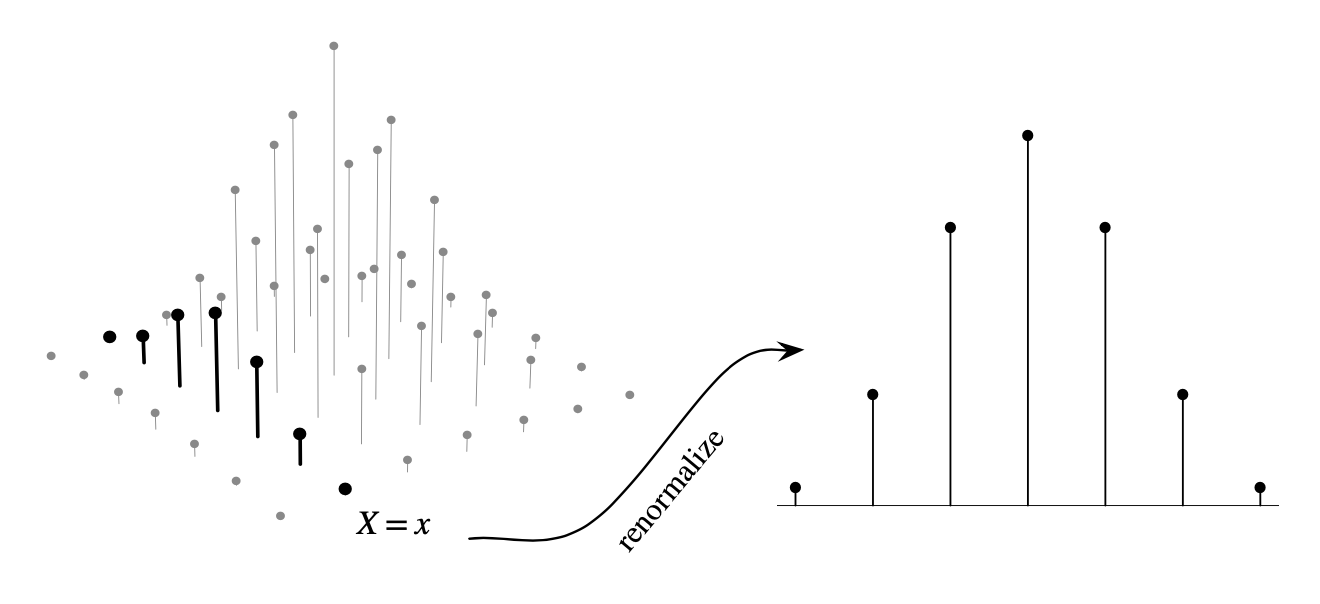
\includegraphics[width=6in]{imgs/conditional_pf.png}
        \caption{Conditional p.f. of $Y$ given $X=x$. This is obtained by starting with the 
        joint p.f (left) column compatible with $X=x$ and then renormalizing by dividing by 
        $P(X=x)$ so the conditional p.f. sums to 1.}
    \end{figure}
\end{itemize}

\textbf{Conditional Probability Density Function}
\begin{itemize}
    \item For continuous r.v.s $X$ and $Y$ with joint p.d.f. $f$ and $X$ with marginal p.d.f. 
    $f_1$, the conditional p.d.f. of $Y$ given $X=x$ is 
    \[g_2(y|x) = \frac{f(x,y)}{f_1(x)}\]
    where $g_2$ is the conditional p.d.f. of $Y$ given $X=x$.
    \begin{figure}[H] 
        \centering 
        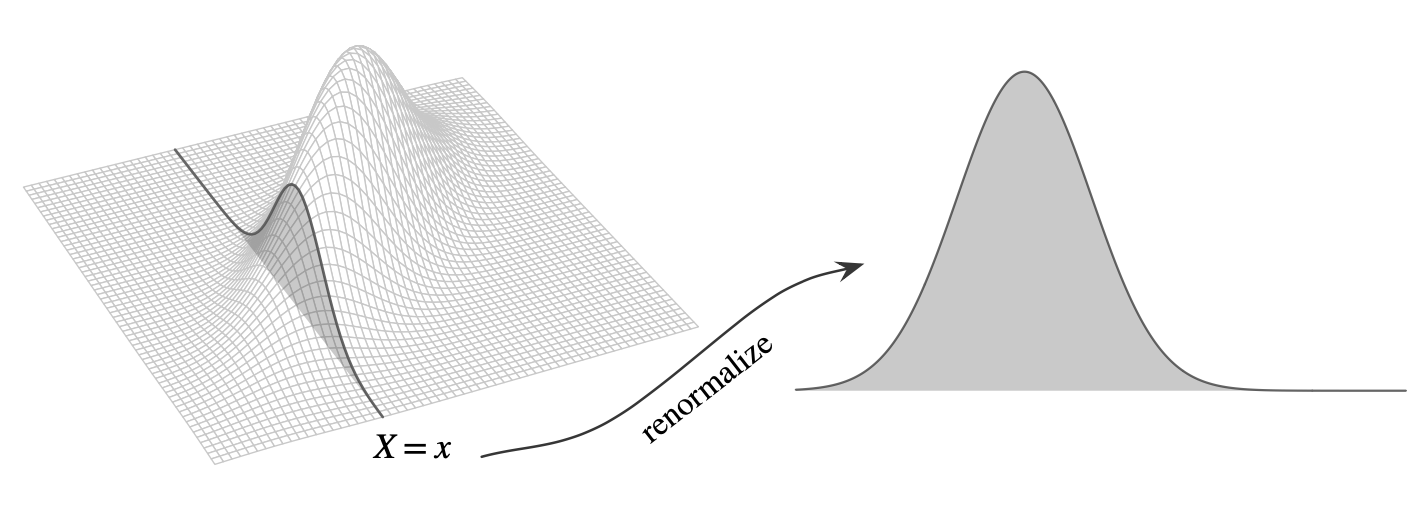
\includegraphics[width=6in]{imgs/conditional_pdf.png}
        \caption{Conditional p.d.f. of $Y$ given $X=x$. This is obtained by starting with the 
        joint p.d.f (left) slice compatible with $X=x$ and then renormalizing by dividing by 
        $P(X=x)$ so the conditional p.d.f. integrates to 1.}
    \end{figure}
    \item It is important to keep in mind that the conditional p.d.f. of $X$ given $Y=y$ is 
    better thought of as the conditional p.d.f. of $X$ given that $Y$ is very close to $y$.
    This motivates us to remember the distinction between the conditional p.d.f. and 
    conditioning on an event with probability 0. 
\end{itemize}

\textbf{Law of Total Probability with Conditional Probabilities}
\begin{itemize}
    \item If $f_2(y)$ is the marginal p.f. or p.d.f. of a r.v. $Y$ and $g_1(x|y)$ is the 
    conditional p.f. or p.d.f. of $X$ given $Y=y$, then the marginal p.f. or p.d.f. of $X$ is
    \[f_1(x) = \sum_y g_1(x|y)f_2(y)\]
    if $Y$ is discrete. If $Y$ is continuous, the marginal p.f. or p.d.f of $X$ is 
    \[f_1(x) = \int_{-\infty}^{\infty} g_1(x|y)f_2(y) \,dy\]
\end{itemize}

\textbf{Bayes' Rule with Conditional Probabilities}
\begin{itemize}
    \item If $f_2(y)$ is the marginal p.f. or p.d.f. of a r.v. $Y$ and $g_1(x|y)$ is the 
    conditional p.f. or p.d.f. of $X$ given $Y=y$, then the conditional p.f. or p.d.f. or $Y$ 
    given $X=x$ is 
    \[g_2(y|x) = \frac{g_1(x|y)f_2(y)}{f_1(x)}\]
    where $f_1(x)$ is obtained the above appropriate LOTP formula.
    \item Similarly, the conditional p.f. or p.d.f. of $X$ given $Y=y$ is 
    \[g_1(x|y) = \frac{g_2(y|x)f_1(x)}{f_2(y)}\]
    where $f_2(y)$ is obtained the above appropriate LOTP formula with $x$ and $y$ switched and
    with the subscripts 1 and 2 switched.
\end{itemize}

\textbf{Independence}
\begin{itemize}
    \item Suppose that $X$ and $Y$ are 2 r.v.s having a joint p.f., p.d.f, or p.f./p.d.f. $f$. 
    Then $X$ and $Y$ are independent if and only if for every value of $y$ such that $f_2(y)
    >0$ and every value of $x$
    \[g_1(x|y)=f_1(x)\]
\end{itemize}

\subsection{Multivariate Distributions}

\textbf{Multivariate Distributions}
\begin{itemize}
    \item Multivariate distributions are simply an extension of the 2 r.v. (bivariate)
    distributions to $n$ r.v. (multivariate) distributions.
    \item In general, the joint distribution of more than 2 r.v.s is called a multivariate 
    distribution.
    \item The theory of statistical inference relies on mathematical models for observable data
    in which each observation is a r.v. Therefore, multivariate distributions arise naturally 
    in the mathematical models for data. 
\end{itemize}

\textbf{Vector Notation}
\begin{itemize}
    \item When dealing with $n$ r.v.s, $X_1, \ldots, X_n$, it is often more convenient to use 
    the vector notation $\boldsymbol{X}=(X_1, \ldots, X_n)$.
    \item $\boldsymbol{X}$ is referred to as a \textit{random vector}.
    \item Instead of speaking of the joint distrubution of the r.v.s $X_1, \ldots, X_n$ with a
    joint c.d.f. $F(x_1, \ldots, x_n)$, we can simply speak of the distribution of the random 
    vector $\boldsymbol{X}$ with c.d.f. $F(\boldsymbol{x})$.
    \item When using vector notation, we must keep in mind that $\boldsymbol{X}$ is an $n$-
    dimensional random vector, with its c.d.f. being defined as a function on the $n$-
    dimensional space $\mathbb{R}^n$.
\end{itemize}

\textbf{Multivariate Discrete Distributions}
\begin{itemize}
    \item $n$ r.v.s $X_1, \ldots, X_n$ have a discrete joint distribution if the random vector 
    $\boldsymbol{X}=(X_1, \ldots, X_n)$ can have only a finite number or an infinite sequence
    of different possible values $(x_1, \ldots, x_n)$ in $\mathbb{R}^n$.
    \item The joint p.f. of $X_1, \ldots, X_n$ is defined as the function $f$ such that for 
    every point $(x_1, \ldots, x_n) \in \mathbb{R}^n$
    \[f(x_1, \ldots, x_n) = P(X_1=x_1, \ldots, X_n=x_n)\]
    \[f(\boldsymbol{x}) = P(\boldsymbol{X}=\boldsymbol{x})\]
    \item If $\boldsymbol{X}$ has a joint discrete distribution with p.f. $f$, then for every 
    subset $C \subset \mathbb{R}^n$
    \[P(\boldsymbol{X} \in C) = \sum_{x \in C} f(\boldsymbol{x})\]
\end{itemize}

\textbf{Multivariate Continuous Distributions}
\begin{itemize}
    \item $n$ r.v.s $X_1, \ldots, X_n$ have a continuous joint distribution if there is a 
    nonnegative function (joint p.d.f. of $\boldsymbol{X}$) $f$ defined on $\mathbb{R}^n$ such 
    that for every subset $C \subset 
    \mathbb{R}^n$
    \[P[(X_1, \ldots, X_n) \in C] = \int \underset{C}{\ldots} \int f(x_1, \ldots, x_n) \,dx_1, 
    \ldots, \,dx_n \]
    \[P(\boldsymbol{X} \in C) = \int \underset{C}{\ldots} \int f(\boldsymbol{x}) \,d
    \boldsymbol{x} \]
    \item Even if each of \(X_1, \ldots, X_n\), has a continuous distribution, the vector 
    \(\boldsymbol{X}\) might not have a continuous joint distribution.
\end{itemize}

\textbf{Multivariate Mixed Distributions}
\begin{itemize}
    \item If $X_1, \ldots, X_n$ are a combindation of discrete and continuous r.v.s, their 
    joint distribution would then be represented by a function $f$, called the \textit{joint
    p.f./p.d.f.}
    \item The function has the property that the probability that $\boldsymbol{X}$ lies in a 
    subset $C \subset \mathbb{R}^n$ is calculated by summing $f(\boldsymbol{x})$ over the 
    values of the coordinates of $\boldsymbol{x}$ that correspond to the discrete r.v.s and 
    integrating over the coordinates that correspond to the continuous r.v.s for all points 
    \(\boldsymbol{x} \in C\).
\end{itemize}

\textbf{Deriving a Marginal p.d.f. from a Multivariate Continuous Distribution}
\begin{itemize}
    \item If the joint distribution of \(n\) r.v.s \(X_1, \ldots, X_n\) is known, then the 
    marginal distributions of each single r.v. \(X_i\) can be derived from this joint 
    distribution.
    \item The marginal joint p.d.f. of any $k$ of the $n$ random variables \(X_1, \ldots, X_n\)
    can be found by integerating the joint p.d.f. over all possible values of the other \(n-k\)
    variables. 
    \item If the joint p.d.f. of \(X_1, \ldots, X_n\) is \(f\), then the marginal p.d.f. 
    \(f_1\) of \(X_1\) is specified at every value \(x_1\) by the relation 
    \[f_1(x_1)=\underbrace{\int_{-\infty}^{\infty} \ldots \int_{-\infty}^{\infty}}_{n-1} f(x_1,
    \ldots, x_n) \,dx_2 \ldots \,dx_n\]
    \item If the joint p.d.f. of \(X_1, X_2, X_3, X_4\) is \(f\), then the marginal bivariate 
    p.d.f. \(f_{24}\) of \(X_2\) and \(X_4\) is specified at each point \((x_2, x_4)\) by the 
    relation 
    \[f_{24}(x_2, x_4)= \int_{-\infty}^{\infty} \int_{-\infty}^{\infty} f(x_1, x_2, x_3, x_4) 
    \,dx_1 \,dx_3\]
\end{itemize}

\textbf{Deriving a Marginal p.f. from a Multivariate Discrete Distribution}
\begin{itemize}
    \item If \(n\) r.v.s \(X_1, \ldots, X_n\) have a discrete joint distribution, then the 
    marginal joint p.f. of each subset of the $n$ variables can be obtained from the relations
    similar to those for continuous distributions where the integrals are replaced by sums.
\end{itemize}

\textbf{Deriving a Marginal c.d.f.}
\begin{itemize}
    \item The marginal joint c.d.f. fo any $k$ of $n$ r.v.s \(X_1, \ldots, X_n\) can be found 
    by computing the limiting value of the $n$-dimensional c.d.f. $F$ as $x_j \to \infty$ for 
    each of the other $n-k$ variables $x_j$. 
    \item If the joint c.d.f. of \(X_1, \ldots, X_n\) is \(F\), then the marginal c.d.f. 
    \(F_1\) of \(X_1\) can be obtained from the following relation
    \[F_1(x_1)=P(X_1 \le x_1) = P(X_1 \le x_1, X_2 < \infty, \ldots, X_n < \infty)\]
    \[F_1(x_1)=\lim_{x_2, \ldots, x_n \to \infty} F(x_1, x_2, \ldots, x_n) \]
    \item If $F$ is the joint c.d.f. of 4 r.v.s $X_1, X_2, X_3, X_4$, then the marginal 
    bivariate c.d.f. $F_{24}$ of $X_2$ and $X_4$ is specified at every point $(x_2, x_4)$ by
    the relation 
    \[F_{24}(x_2, x_4) = \lim_{x_1, x_3 \to \infty} F(x_1, x_2, x_3, x_4)\]
\end{itemize}

\textbf{Independent Random Variables}
\begin{itemize}
    \item $n$ r.v.s $X_1, \ldots, X_n$ are independent if, for every $n$ sets $A_1, \ldots, 
    A_n$ of real numbers 
    \[P(X_1 \in A_1, \ldots, X_n \in A_n) = P(X_1 \in A_1) \ldots P(X_n \in A_n)\]
    \item Let $F$ denote the joint c.d.f. of $X_1, \ldots, X_n$ and let $F_i$ denote the 
    marginal univariate c.d.f. of $X_i$ for $i = 1, \ldots, n$. The variables $X_1, \ldots, 
    X_n$ are independent if and only if, for all points $(x_1, \ldots, x_n) \in \mathbb{R}^n$
    \[F(x_1, \ldots, x_n) = F_1(x_1) \ldots F_n(x_n)\]
    \item If $X_1, \ldots, X_n$ have a continuous, discrete, or mixed joint distribution for 
    which the joint p.d.f., joint p.f., or joint p.f./p.d.f. is $f$, and if $f_i$ is the 
    marginal univariate p.d.f. or p.f. of $X_i$ for $i = 1, \ldots, n$, then $X_1, \ldots X_n$
    are independent if and only if the following relation is satisfied at all points $x_1, 
    \ldots, x_n \in \mathbb{R}^n$
    \[f(x_1, \ldots, x_n)=f_1(x_1) \ldots f_n(x_n)\]
    \item Consider a given probability distribution of the real line that can be represented 
    by either a p.f. or a p.d.f. $f$. It is said that $n$ r.v.s $X_1, \ldots X_n$ form a 
    \textit{random sample} from this distribution if these r.v.s are independent and the 
    marginal p.f. or p.d.f. of each of them is $f$. Such r.v.s are also said to be \textit{
    independent and identically distributed (i.i.d.)}. We refer to the number $n$ of r.v.s as 
    the \textit{sample size}.
    \item $n$ r.v.s $X_1, \ldots, X_n$ each with marginal p.f./p.d.f. $f$ and joint 
    distribution $g$ if and only if, at all points $(x_1, \ldots, x_n) \in \mathbb{R}^n$
    \[g(x_1, \ldots, x_n) = f(x_1) \ldots f(x_n)\]
    
    \textbf{Conditional Multivariate Distributions}
    \begin{itemize}
        \item Suppose that $n$ r.v.s $X_1, \ldots, X_n$ have a continuous distribution for 
        which the joint p.d.f. is $f$ and that $f_0$ denotes the marginal joint p.d.f. of the
        $k < n$ r.v.s $X_1, \ldots, X_k$. Then for all values of $x_1, \ldots x_k$ such that 
        $f_0(x_1, \ldots, x_k) > 0$, the conditional p.d.f. of $(X_{k+1}, \ldots X_n)$ given 
        that $X_1=x_1, \ldots, X_k=x_k$ is defined as 
        \[g_{k+1 \ldots n}(x_{k+1}, \ldots x_n | x_1, \ldots x_k) = \frac{f(x_1, \ldots x_n)}
        {f_0(x_1, \ldots, x_k)}\]
        \item More generally, suppose that the random vector $\boldsymbol{X}=(X_1, \ldots X_n)
        $ is divided into 2 subvectors $\boldsymbol{Y}$ and $\boldsymbol{Z}$ where 
        $\boldsymbol{Y}$ is a $k$-dimensional random vector comprising $k$ of the $n$ r.v.s in 
        $\boldsymbol{X}$, and $\boldsymbol{Z}$ is an $(n-k)$-dimensional random vector 
        comprising of the other $n-k$ random variables in $\boldsymbol{X}$. Suppose also that 
        the $n$-dimensional joint p.f., p.d.f., or p.f./p.d.f. of $(\boldsymbol{Y}, 
        \boldsymbol{Z})$ is $f$ and that the marginal $(n-k)$-dimensional p.f., p.d.f., or
        p.f./p.d.f. of $\boldsymbol{Z}$ is $f_2$. Then for every given point $\boldsymbol{z}
        \in \mathbb{R}^{n-k}$ such that $f_2(\boldsymbol{z})>0$, the conditional $k$
        -dimensional p.f., p.d.f., or p.f./p.d.f. $g_1$ of $\boldsymbol{Y}$ given 
        $\boldsymbol{Z} = \boldsymbol{z}$ is defined as 
        \[g_1(\boldsymbol{y}|\boldsymbol{z}) = \frac{f(\boldsymbol{y}, \boldsymbol{z})}
        {f_2(\boldsymbol{z})}\]
        for $\boldsymbol{y} \in \mathbb{R}^k$. \\

        This can be rewritten as
        \[f(\boldsymbol{y}, \boldsymbol{z}) = g_1(\boldsymbol{y}|\boldsymbol{z})f_2(
        \boldsymbol{z})\]
        \item To determine the conditional version given $\boldsymbol{W} = \boldsymbol{w}$ of 
        a result just proven, simply add conditional on $\boldsymbol{W} = \boldsymbol{w}$ to 
        every probabilistic statement in the result. 
    \end{itemize}

    \textbf{Multivariate Law of Total Probability and Bayes' Theorem}
    \begin{itemize}
        \item Suppose that the random vector $\boldsymbol{X}=(X_1, \ldots X_n)
        $ is divided into 2 subvectors $\boldsymbol{Y}$ and $\boldsymbol{Z}$ where 
        $\boldsymbol{Y}$ is a $k$-dimensional random vector comprising $k$ of the $n$ r.v.s in 
        $\boldsymbol{X}$, and $\boldsymbol{Z}$ is an $(n-k)$-dimensional random vector 
        comprising of the other $n-k$ random variables in $\boldsymbol{X}$. Suppose also that 
        the $n$-dimensional joint p.f., p.d.f., or p.f./p.d.f. of $(\boldsymbol{Y}, 
        \boldsymbol{Z})$ is $f$ and that the marginal $(n-k)$-dimensional p.f., p.d.f., or
        p.f./p.d.f. of $\boldsymbol{Z}$ is $f_2$. If $\boldsymbol{Z}$ has a continuous joint
        distribution, the marginal p.d.f. of $\boldsymbol{Y}$ is 
        \[f_1(\boldsymbol{y})= \underbrace{\int_{-\infty}^{\infty} \ldots \int_{-\infty}^{
        \infty} }_{n-k} g_1(\boldsymbol{y}|\boldsymbol{z})f_2(\boldsymbol{z})\,d
        \boldsymbol{z}\]
        and the conditional p.d.f. of $\boldsymbol{Z}$ given $\boldsymbol{Y}=\boldsymbol{y}$ 
        is
        \[g_2(\boldsymbol{z}|\boldsymbol{y})=\frac{g_1(\boldsymbol{y}|\boldsymbol{z})f_2(
        \boldsymbol{z})}{f_1(\boldsymbol{y})}\]
        \item If $\boldsymbol{Z}$ has a discrete distribution, then the multiple integreal 
        must be replaced with a multiple summation. 
    \end{itemize}

    \textbf{Conditionally Independent Random Variables}
    \begin{itemize}
        \item Let $\boldsymbol{Z}$ be a random vector with joint p.f., p.d.f., or p.f./p.d.f.
        $f_0(\boldsymbol{z})$. Several random variables $X_1, \ldots, X_n$ are \textit{
        conditionally independent} given $\boldsymbol{Z}$ if, for all $\boldsymbol{z}$ such 
        that $f_0(\boldsymbol{z})>0$, we have 
        \[g(\boldsymbol{x}|\boldsymbol{z})= \prod_{i=1}^{n}g_i(x_i|\boldsymbol{z})\]
    \end{itemize}
\end{itemize}

\subsection{Functions of a Random Variable}

\textbf{Why Functions of a Random Variable Are Important}
\begin{itemize}
    \item Often we find after computing the distribution of a r.v. $X$, we actually want to 
    find the distribution of some function of $X$.
    \item An example is if $X$ is the rate at which customers are served in a queue, but we 
    want the average waiting time, defined as $Y = 1/X$.
    \item Having the distribution of $X$ is enough to find the distribution of some function 
    of $X$.
\end{itemize}

\textbf{Deriving a p.f. for a Function of a Discrete Random Variable}
\begin{itemize}
    \item Let $X$ have a discrete distribution with p.f. $f$, and let $Y=r(X)$ for some 
    function of $r$ defined on the set of possible values of $X$. For each possible value $y$
    of $Y$, the p.f. $g$ of $Y$ is

    \[g(y) = P(Y=y) = P[r(X)=y] = \sum_{x:r(x)=y} f(x)\]

    which says that the $P(Y=y)$ is equal to the summation of the probabilities of all values 
    where $r(x)=y$. In other words, for some value of $y$, we see all the values where $r(x)
    =y$ and sum over each probability, that is, for each $P(X=x)$.

    \item Example
    \begin{itemize}
        \item Let $X$ have the uniform distribution on integers $1, \ldots, 9$.
        \item Suppose we are interested in how far $X$ is from the middle of the distribution, 
        namely, 5. 
        \item We can define $Y= |X-5|$ and compute probabilities. For example, we could 
        compute $P(Y=1) = P(X=4 \cup X=6) = \frac{1}{9} + \frac{1}{9} = \frac{2}{9}$ (here, 
        $r(x)=y$ exactly when $x=4$ or $x=6$).
    \end{itemize}
\end{itemize}

\textbf{Deriving a c.d.f. for a Function of a Continuous Random Variable}
\begin{itemize}
    \item The process for deriving the probability distribution for a continuous r.v. differs
    from the procedure for deriving the probability distribution for a discrete r.v. 
    \item Suppose that a continuous r.v. $X$ with a p.d.f. $f$ and another continuous r.v. $Y$
    is defined as $Y=r(X)$. For each real number $y$, the c.d.f., $G(y)$ of $Y$ can be derived
    as 
    \[G(y) = P(Y \le y) = P[r(X) \le y] = \int_{{x:r(x) \le y}} f(x) \,dx \]

    which says that $P(Y \le y)$ is equal to the integral of the p.d.f. of $x$ for all values 
    where $r(x) \le y$.
\end{itemize}

\textbf{Deriving a p.d.f. for a Function of a Continuous Random Variable}
\begin{itemize}
    \item Suppose that a continuous r.v. $X$ with a p.d.f. $f$ and another continuous r.v. $Y$
    is defined as $Y=r(X)$. The p.d.f. of $Y$, defined as $g$, can be obtained from the 
    relation
    \[g(y) = \frac{d}{dy} G(y)\]
    \item Example 
    \begin{itemize}
        \item For 2 continuous r.v.s $X$ and $Y$, derive the p.d.f. for $Y=X^2$ when $X$ has
        the uniform distribution on the interval $[-1,1]$, so
        \[
        \begin{cases}
            1/2 & \text{for } -1 \le x \le 1 \\
            0 & \text{otherwise}
        \end{cases}    
        \]
    \end{itemize}
    To find the p.d.f. of $Y$, we will first find the c.d.f. of $Y$ and then use the c.d.f. to 
    find the p.d.f.
    Since $Y=X^2$, then $Y$ must belong to the interval $0 \le Y \le 1$. Thus, for each value 
    of $Y$ such that $0 \le Y \le 1$, the c.d.f. $G(y)$ of $Y$ is 
    
    \[G(y) = P(Y \le y) = P[r(X) \le y] = \int_{{x:r(x) \le y}} f(x) \,dx \]
    \[G(y) = P(Y \le y) = P[r(X) \le y] = P[X^2 \le y] = P(-\sqrt{y} \le X \le \sqrt{y}) =\] 
    \[\int_{-\sqrt{y}}^{\sqrt{y}} 1/2 \,dx = \frac{1}{2}x |_{-\sqrt{y}}^{\sqrt{y}} = 
    \frac{\sqrt{y}}{2} - -\frac{\sqrt{y}}{2} = \sqrt{y}\]
    
    Now to find the p.d.f. of $Y$
    \[g(y) = \frac{d}{dy} G(y)\]
    \[g(y) = \frac{d}{dy} \sqrt{y} = \frac{1}{2\sqrt{y}}\]
\end{itemize}

\subsection{Functions of Two or More Random Variables}

\textbf{Why Functions of Two or More Random Variables are Important}
\begin{itemize}
    \item When observing data consisting of the values of several r.v.s, we need to summarize 
    the observed values in order to be able to focus on the information in the data. 
    \item Sumamrizing consists of constructing 1 or a few functions of the r.v.s that capture
    the bulk of the information. 
\end{itemize}

\textbf{Deriving a Joint p.f. for a Function of Discrete Random Variables}
\begin{itemize}
    \item Suppose that $n$ r.v.s $X_1, \ldots, X_n$ have a discrete joint distribution for 
    which the joint p.f. is $f$, and that $m$ functions $Y_1, \ldots, Y_m$ of these $n$ r.v.s
    are defined as 
    \begin{align*}
        Y_1 &= r_1(X_1, \ldots, X_n) \\
        Y_2 &= r_2(X_1, \ldots, X_n) \\
        \vdots \\
        Y_m &= r_m(X_1, \ldots, X_n)
    \end{align*}

    for given values $y_1, \ldots, y_m$ of the $m$ r.v.s $Y_1, \ldots, Y_m$, let $A$ denote
    the set of all points $(x_1, \ldots, x_n)$ such that

    \begin{align*}
        y_1 &= r_1(x_1, \ldots, x_n) \\
        y_2 &= r_2(x_1, \ldots, x_n) \\
        \vdots \\ 
        y_m &= r_m(x_1, \ldots, x_n)
    \end{align*}

    then the value of the joint p.f. $g$ of $Y_1, \ldots, Y_m$ is specified at the point 
    $(y_1, \ldots, y_m)$ by the relation 

    \[g(y_1, \ldots, y_m) = \sum_{(x_1, \ldots, x_n) \in A} f(x_1, \ldots, x_n)\]

    In words, this says that the joint p.f. of $g(y_1, \ldots y_m)$ is equal to the summation 
    of the probabilities of all the values where $r(\boldsymbol{x})= \boldsymbol{y}$. In other 
    words, for some value of $\boldsymbol{y}$, where $\boldsymbol{y}$ is a vector, we see all 
    the values where $r(\boldsymbol{x})= \boldsymbol{y}$ and sum over each probability.

    \item Example 
    \begin{itemize}
        \item Suppose 3 different investment firms are trying to advertise their mutual funds 
        by showing how many perform better than the market. Each company has 10 funds, so 
        there are 30 in total. Suppose the first 10 funds belong to firm 1, the second 10 to
        firm 2, and the last 10 to firm 3. Let $X_i=1$ if fund $i$ performs better than the 
        market and $X_i=0$ otherwise, for $i=1, \ldots, 30$. Then, we are interested in 3 
        functions
        \begin{align*}
            Y_1 &= X_{1}+ \cdots + X_{10} \\
            Y_2 &= X_{11} + \cdots + X_{20} \\
            Y_3 &= X_{21} + \cdots + X_{30}
        \end{align*}

        and we would like to determine the joint p.f. $g$ of $(Y_1, Y_2, Y_3)$ at the point 
        $(3, 5, 8)$. That is, we want $g(3,5,8)=P(Y_1=3, Y_2=5, Y_3=8)$.

        \item We define the set $A$ as 
        \[ A = \{ (x_1, \ldots, x_{30}): x_1 + \cdots + x_{10} = 3, x_{11} + \cdots + x_{20} = 5
        , x_{21} + \cdots + x_{30} = 8 \} \]

        \item The amount of points in the set $A$ are 
        \[ {10 \choose 3} {10 \choose 5} {10 \choose 8} = 1,360,800 \]

        \item If we assume that all $2^{30}$ possible values of the vector $(X_1, \ldots, 
        X_{30})$ are equally likely (big assumption), then 
        \[ g(3,5,8) = \frac{1,360,800}{2^{30}} = 1.26 \times 10^{-3} \]
    \end{itemize}

    \textbf{Binomial and Bernoulli Distributions}
    \begin{itemize}
        \item Assume that $X_1, \ldots, X_n$ are i.i.d. r.v.s having the Bernoulli 
        distribution with parameter $p$. Let $Y = X_1 + \cdots + X_n =$. Then $Y$ has the 
        binomial distribution with parameters $n$ and $p$.
    \end{itemize}
\end{itemize}

\textbf{Deriving a c.d.f. for a Function of Countinuous Random Variables}
\begin{itemize}
    \item Suppose that the joint p.d.f. of $\boldsymbol{X} = (X_1, \ldots, X_n)$ is 
    $f(\boldsymbol{x})$ and that $Y = r(\boldsymbol{X})$. For each real number $y$, define 
    $A_y = \{ \boldsymbol{x}: r(\boldsymbol{x} \le y) \}$. Then the c.d.f. $G(y)$ of $Y$ is 
    \[ G(y) = \int \underset{A_y}{\ldots} \int f(\boldsymbol{x}) \,d\boldsymbol{x}\]
\end{itemize}

\textbf{Convolution}
\begin{itemize}
    \item A \textit{convolution} is a sum of independent r.v.s.
    \item Let $X_1$ and $X_2$ by independent continuous r.v.s and let $Y=X_1+X_2$. The 
    distribution of $Y$ is called the \textit{convolution} of the distributions of $X_1$ and 
    $X_2$. The p.d.f. of $Y$ is sometimes called the convolution of the p.d.f.'s of $X_1$ and 
    $X_2$.
\end{itemize}

\subsection{Markov Chains}

\textbf{Markov Chains Basics}
\begin{itemize}
    \item A Markov chain model is a popular model for systems that change over time in a 
    random manner.
    \item A Markov chain is a sequence of r.v.s, one for each time period. 
    \item At each time period, the corresponding r.v. gives the state of the system.
    \item The conditional distribution of each future state given the past states and the 
    present state depends on the present state. 
\end{itemize}

\textbf{Stochastic Processes}
\begin{itemize}
    \item A sequence of r.v.s $X_1, X_2, \ldots$ indexed by time is called a 
    \textit{stochastic process} or \textit{random process} with discrete time parameter. 
    \item The first r.v. $X_1$ is called the \textit{initial state} of the process; and for 
    $n=2, 3, \ldots$, the r.v. $X_n$ is called the \textit{state of the process at time} $n$.
    \item A discrete time parameter means that the process is only observed at discrete or 
    separated points in time (such as at 2 minute intervals) instead of continuously in time.
    \item Example 
    \begin{itemize}
        \item For an office with 5 telephone lines, let $X_n$ for $n=1, 2, \ldots$ denote the 
        number of lines being used at time $n$ (where each $n$ is observed at 2 minute 
        intervals). 
        \item The state of the process at any time is the number of lines being used at that 
        time. Therefore, it must take a value between 0 and 5. 
    \end{itemize}
    \item To describe the complete probability model for a particular process, it is necessary 
    to specify the distribution for the initial state $X_1$ and also to specify for each $n=1,
    2, \ldots$ the conditional distribution of the subsequent state $X_{n+1}$ given $X_1, 
    \ldots X_n$. These conditional distributions are equivalent to the collection of 
    conditional c.d.f.s of the following form 
    \[ P(X_{n+1} \le b | X_1 = x_1, \ldots, X_n = x_n) \]
\end{itemize}

\textbf{Markov Chains}
\begin{itemize}
    \item A Markov chain is a special type of stochastic process, defined in terms of the 
    conditional distributions of future states given the present and past states. 
    \item A stochastic process with discrete time parameter is a \textit{Markov chain} if, for
    each time $n$, the conditional distributions of all $X_{n+j}$ for $j \ge 1$ given $X_1, 
    \ldots, X_n$ depend only on $X_n$ and not on the earlier states $X_1, \ldots, X_{n-1}$. In 
    symbols, for $n=1, 2, \ldots$ and for each $b$ and each possible sequence of states $x_1, 
    \ldots, x_n$ 
    \[ P(X_{n+1} \le b | X_1=x_1, \ldots, X_n=x_n) = P(X_{n+1} \le b | X_n = x_n)\]

    which means that the conditional distribution of some state only depends on the state 
    immediately prior. 
    \item A Markov chain is called finite if there are only finitely many possible states. 
    \item For a finite Markov chain, the joint p.f. for the first $n$ states is 
    \[ P(X_n=x_n | X_{n-1}= x_{n-1}) \]
\end{itemize}

\textbf{Transition Distributions/Stationary Transition Distributions}
\begin{itemize}
    \item Consider a finite Markov chain with $k$ possible states. The conditional 
    distributions of the state at time $n+1$ given the states at time $n$, that is $P(X_{n+1}
    = j | X_n = i)$ for $i,j = 1, \ldots, k$ and $n = 1, 2, \ldots$ are called the \textit{
    transition distributions} of the Markov chain. 
    \item If the distribution is the same for every time $n$ $(n=1, 2, \ldots)$, then the 
    Markov chain has \textit{stationary transition distributions}.
\end{itemize}

\section{Expectation}

\subsection{The Expectation of a Random Variable}

\textbf{Why Expectation is Important}
\begin{itemize}
    \item Although the distribution of a r.v. $X$ contains all the probabilistic information 
    about $X$, it is often too cumbersome to present the entire distribution of $X$.
    \item Instead, we can summarize the data in multiple ways. One such way is to summarize 
    what the average, or expected value, of $X$ we expect to see.
\end{itemize}

\textbf{Expectation Basics}
\begin{itemize}
    \item The intuitive idea of the mean of a r.v. is that it is the weighted average of the 
    possible values of the r.v. with the weights equal to the probabilities.
    \item The expectation of $X$ depends only on the distribution of $X$.
    \item The expectation of a r.v., or equivalently, the mean of its distribution can be 
    regarded as being the center of gravity of that distribution. 
    \item Can be affected greatly by even a very small change in the amount of probability 
    that is assigned to a very large value of $x$. 
\end{itemize}

\textbf{Expectation for a Discrete Distribution}
\begin{itemize}
    \item Let $X$ be a bounded discrete r.v. whose p.f. is $f$. The \textit{expectation} of 
    $X$, denoted $E(X)$, is a number defined as 
    \[E(X) = \sum_{\text{All } x}x f(x)\]
\end{itemize}

\textbf{Expectation for a Continuous Distribution}
\begin{itemize}
    \item Let $X$ be a bounded continuous r.v. whose p.d.f. is $f$. The \textit{expectation} 
    of $X$, denoted $E(X)$, is a number defined as 
    \[E(X) = \int_{\text{All } x}x f(x) \,dx\]
\end{itemize}

\textbf{Law of the Unconscious Statistician (1-D)}
\begin{itemize}
    \item 1-D LOTUS provides a method to find $E(g(X))$ directly using the distribution of $X$ 
    without having to find the distribution of $g(X)$.
    \item The name comes from the fact that going from $E(X)$ to $E(g(X))$ it is tempting to 
    just change $x$ to $g(x)$ in the definition, which can be done very easily and 
    mechanically, perhaps in a state of unconsciousness. Although it may sound too good to be 
    true, but LOTUS says it is true. 
    \item If $X$ has a continuous distribution, then LOTUS says
    \[E(g(X)) = \int_{-\infty}^{\infty} g(x) f(x) \,dx\]
    \item If $X$ has a discrete distribution, then LOTUS says
    \[E(g(X)) = \sum_{\text{All } x} g(x) f(x)\]
\end{itemize}

\textbf{Law of the Unconscious Statistician (2-D)}
\begin{itemize}
    \item 2-D LOTUS provides a method to find $E(g(X,Y))$ directly using the joint 
    distribution of $X$ and $Y$ without having to find the distribution of $g(X,Y)$.
    \item If $X$ and $Y$ are continuous with joint p.d.f $f(x,y)$, then LOTUS says
    \[E(g(X,y)) = \int_{-\infty}^{\infty} \int_{-\infty}^{\infty} g(x,y) f(x,y) \,dx \,dy\]
    \item If $X$ and $Y$ are discrete with joint p.f. $f(x,y)$, then LOTUS says
    \[E(g(X)) = \sum_{\text{All } x} \sum_{\text{All } y} g(x,y) f(x,y)\]
    \item 2-D LOTUS easily extends to $n$-D LOTUS.
\end{itemize}

\subsection{Properties of Expectations}
\subsection{Variance}
\subsection{Moments}
\textbf{Moments Basics}
\begin{itemize}
    \item They have useful properties and some moments can be used for additional summaries of 
    a distribution. 
\end{itemize}

\textbf{Raw Moments}
\begin{itemize}
    \item For each r.v. $X$ and every positive integer $k$, the expectation $E(X^k)$ is called 
    the $k$th \textit{raw moment} of $X$.
    \item Notably, following raw moments, the mean of $X$ is the first moment of $X$.
    \item First Four Raw Moments
    \begin{enumerate}
        \item $E(X)=\frac{\sum_{i=1}^{n} x_i}{n}$
        \item $E(X^2)=\frac{\sum_{i=1}^{n} x_i^2}{n}$
        \item $E(X^3)=\frac{\sum_{i=1}^{n} x_i^3}{n}$
        \item $E(X^4)=\frac{\sum_{i=1}^{n} x_i^4}{n}$
    \end{enumerate}
\end{itemize}

\textbf{Existence of Moments}
\begin{itemize}
    \item The $k$th moment exists if and only if $E({|X|}^k) < \infty$
    \item If $E({|X|}^k) < \infty$ for some positive integer $k$, then $E({|X|}^j) < \infty$ 
    for every positive integer $j$ such that $j < k$. In other words, if we know the $k$th 
    moment exists, then we know all moments prior to $k$ also exist.
\end{itemize}

\textbf{Centered Moments}
\begin{itemize}
    \item Suppose that $X$ is a r.v. for which $E(X)=\mu$. For every positive integer $k$, the 
    expectation $E[{(X-\mu)}^k]$ is called the $k$th \textit{central moment} of $X$ about the 
    mean.
    \item Subtracting the mean, we are effectively netting out the effect of the first moment.
    \item Notably, following central moments, the variance of $X$ is the second moment of $X$.
    \item First Four Central Moments
    \begin{enumerate}
        \item $E[(X-\mu)]=\frac{\sum_{i=1}^{n} (x_i-\mu)}{n}=0$
        \item $E[{(X-\mu)}^2]=\frac{\sum_{i=1}^{n} {(x_i-\mu)}^2}{n}$
        \item $E[{(X-\mu)}^3]=\frac{\sum_{i=1}^{n} {(x_i-\mu)}^3}{n}$
        \item $E[{(X-\mu)}^4]=\frac{\sum_{i=1}^{n} {(x_i-\mu)}^4}{n}$
    \end{enumerate}
\end{itemize}

\textbf{Standardized Moments}
\begin{itemize}
    \item Let $X$ be a r.v. with mean $\mu$, standard deviation $\sigma$, and finite third 
    moment. The \textit{skewness} of $X$  is defined to be $\frac{E[{(X-\mu)}^3]}{\sigma^3}$
    \item Dividing the third central moment by $\sigma^3$ nets out the effect of the first and 
    second moment. It makes the skewness measure only the lack of symmetry rather than the 
    spread of the distribution. 
    \item Notably, following standardized moments, the skewness of $X$ is the third moment of 
    $X$ and the kurtosis is the fourth moment of $X$.
    \item First Four Standardized Moments
    \begin{enumerate}
        \item $E[(X-\mu)]/\sigma=\frac{\sum_{i=1}^{n} (x_i-\mu)}{n\sigma}=0$
        \item $E[{(X-\mu)}^2]/\sigma^2=\frac{\sum_{i=1}^{n} {(x_i-\mu)}^2}{n\sigma^2}=0$
        \item $E[{(X-\mu)}^3]/\sigma^3=\frac{\sum_{i=1}^{n} {(x_i-\mu)}^3}{n\sigma^3}$
        \item $E[{(X-\mu)}^4]/\sigma^4=\frac{\sum_{i=1}^{n} {(x_i-\mu)}^4}{n\sigma^4}$
    \end{enumerate}
\end{itemize}

\textbf{Sampling Adjustments for the First Three Moments}
\begin{enumerate}
    \item $E(X)=\frac{\sum_{i=1}^{n} x_i}{n}$
    \item $E[{(X-\mu)}^2]=\frac{\sum_{i=1}^{n} {(x_i-\mu)}^2}{n} \to \frac{\sum_{i=1}^{n} {(x_i-\bar{x})}^2}{n-1}$
    \item $E[{(X-\mu)}^3]/\sigma^3=\frac{\sum_{i=1}^{n} {(x_i-\mu)}^3}{n\sigma^3} \to \frac{n}{(n-1)(n-2)}\frac{\sum_{i=1}^{n} {(x_i-\bar{x})}^3}{s^3}$
\end{enumerate}

\textbf{Moment Generating Functions}
\begin{itemize}
    \item A m.g.f. is a generating function that encodes the moments of a distribution.
    \item A distribution is fully characterized by its m.g.f. (same information as from c.d.f.
    or p.d.f.).
\end{itemize}


\section{Special Distributions}
\section{Large Random Samples}

\section{Estimation}

\end{document}
